%%%%%%%%%%%%%%%%%%%%%%%%%%%%%%%%%%%%%%%%%
%
% (c) 2024 by Jennifer Laaser
%
% This work is licensed under the Creative Commons Attribution-NonCommercial-ShareAlike 4.0 International License. To view a copy of this license, visit http://creativecommons.org/licenses/by-nc-sa/4.0/ or send a letter to Creative Commons, PO Box 1866, Mountain View, CA 94042, USA.
%
% The current source for these materials is accessible on Github: https://github.com/jlaaser/pogil-polymers
%
%%%%%%%%%%%%%%%%%%%%%%%%%%%%%%%%%%%%%%%%%

%\documentclass[instructor,handout]{pogil}
\documentclass[handout]{pogil}

%%%%%%%%%%%%%%%%% DOCUMENT INFORMATION %%%%%%%%%%%%%%%%%%%%%%%%

\copyrightshort{
\includegraphics[width=0.1\textwidth]{by-nc-sa} J. Laaser 2024}

%%%%%%%%%%%%%%%%%%%%%%%%%%%%%%%%%%%%%%%%%%%%%%%%%%%%%%%%%%%%%%%%%
%%%%%%%%%%%%%%%%%%%%%%%%%%%%%%%%%%%%%%%%%%%%%%%%%%%%%%%%%%%%%%%%%

\begin{document}
	
% to change the activity output in the pdf, change this to the file path for the activity you want to include:
%%%%%%%%%%%%%%%%%%%%%%%%%%%%%%%%%%%%%%%%%%
%
% (c) 2018 by Jennifer Laaser
%
% This work is licensed under the Creative Commons Attribution-NonCommercial-ShareAlike 4.0 International License. To view a copy of this license, visit http://creativecommons.org/licenses/by-nc-sa/4.0/ or send a letter to Creative Commons, PO Box 1866, Mountain View, CA 94042, USA.
%
% The current source for these materials is accessible on Github: https://github.com/jlaaser/pogil-polymers
%
%%%%%%%%%%%%%%%%%%%%%%%%%%%%%%%%%%%%%%%%%

\section{Activity Template}
\renewcommand{\figpath}{content/figs}

\textbf{Focus question:} Put a central question for the students to consider through this exercise here.

\subsection{Model 1:  ABC}

Here is the first model for students to consider

% to include images, put them in the folder specified by figpath and then use:
%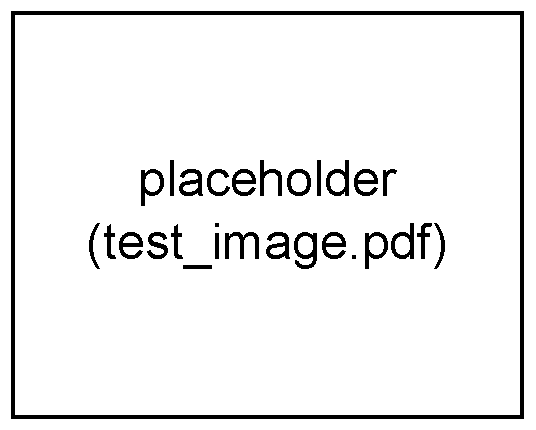
\includegraphics[width=0.8\textwidth]{\figpath/test_image.pdf}

\subsection{Critical Thinking Questions}

	\begin{enumerate}
		\item First question?
		\item Second question?
	\end{enumerate}

\subsection{Model 2: DEF}

\subsection{Critical Thinking Questions}

	\begin{enumerate}
		\item First question?
		\item Second question?
	\end{enumerate}

\subsection{Exercises}

	After class, \textbf{read} the following sections of your textbook:
	
	\begin{enumerate}
		\item First section
		\item Second section
	\end{enumerate}
	
	Then, do the following exercises:
	
	\begin{enumerate}
		\item First exercise
		\item Second exercise
	\end{enumerate}
%%%%%%%%%%%%%%%%%%%%%%%%%%%%%%%%%%%%%%%%%
%
% (c) 2022 by Jennifer Laaser
%
% This work is licensed under the Creative Commons Attribution-NonCommercial-ShareAlike 4.0 International License. To view a copy of this license, visit http://creativecommons.org/licenses/by-nc-sa/4.0/ or send a letter to Creative Commons, PO Box 1866, Mountain View, CA 94042, USA.
%
% The current source for these materials is accessible on Github: https://github.com/jlaaser/pogil-polymers
%
%%%%%%%%%%%%%%%%%%%%%%%%%%%%%%%%%%%%%%%%%

\renewcommand{\figpath}{content/polymphys/scattering/scattering-fundamentals/figs}
\renewcommand{\labelbase}{scattering-fundamentals}

\begin{activity}{Fundamentals of Scattering}
\label{\labelbase}

\begin{instructornotes}
	This activity introduces students to fundamental concepts related to scattering of particles and electromagnetic waves.
	
	After completing this activity, students will be able to:
	\begin{enumerate}
		\item Explain how scattering signals arise from constructive and destructive interference of waves
		\item Relate scattering angles and q vectors to the spacings between particles
		\item Identify types of scattering experiments used in polymer science, and the length scales that they are most suitable for characterizing
	\end{enumerate}
	
	\subsection*{Activity summary:}
	\begin{itemize}
		\item \textbf{Activity type:} Learning Cycle
		\item \textbf{Content goals:} See above
		\item \textbf{Process goals:} %https://pogil.org/uploads/attachments/cj54b5yts006cklx4hh758htf-process-skills-official-pogil-list-2015-original.pdf
			\begin{enumerate}
				\item Interpretation of graphical data
				\item Written and oral communication of reasoning
			\end{enumerate}
		\item \textbf{Duration:} 50 minutes, including time for class discussion
		\item \textbf{Instructor preparation required:} none beyond knowledge of relevant content
		\item \textbf{Related textbook chapters:}
			\begin{itemize}
				\item \emph{Polymer Chemistry} (Hiemenz \& Lodge): sections 8.1 and 8.2
				\item \emph{Introduction to Polymers} (Young \& Lovell): chapter 12 (but minimal coverage of fundamentals - focuses mostly on SLS and DLS)
			\end{itemize}
		\item \textbf{Instructor notes:}
			\begin{itemize}
				\item CTQ \ref{\labelbase:ctq:calcrranges} requires a fair amount of calculation, and can be a little slow.  For efficiency, suggest students split the work up within their group (or, have each group do the calculation for a different experiment and put their answers on the board for everyone to reference as they answer CTQ \ref{\labelbase:ctq:exptchoices})
			\end{itemize}
	\end{itemize}
	
\end{instructornotes}



\begin{model}[Interference of Electromagnetic Waves]
	\label{\labelbase:mdl:interference}
	
	Electromagnetic waves, such as light and X-rays, consist of oscillating electric and magnetic fields propagating through space.
	The electric field, $E$, of an electromagnetic wave propagating along the $x$ axis is shown below:
	
	\vspace{6pt}
	\centerline{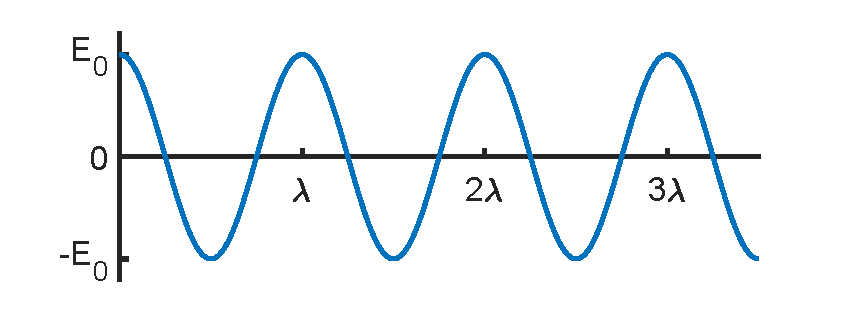
\includegraphics[width=0.7\textwidth]{\figpath/Model1_Ecosx.pdf}}
	
\end{model}


\begin{ctqs}

	\question What is the maximum value of the electric field (the \emph{amplitude} of the electric field) for the wave shown in Model \ref{\labelbase:mdl:interference}?
	
		\begin{solution}[0.25in]{}
			$E_0$
		\end{solution}
	
	\question At what values of $x$ is the amplitude of the wave at this maximum value?
	
		\begin{solution}[0.25in]{}
			0, $\lambda$, $2\lambda$, $3\lambda$
		\end{solution}
	
	\question How much does $x$ have to be increase to move from one maximum of the wave to the next?
	
		\begin{solution}[0.25in]{}
			$\lambda$
		\end{solution}
	
	\question Explain, in 1-2 complete sentences, why $\lambda$ is referred to as the \emph{wavelength} of the wave.
	
		\begin{solution}[1in]{}
			$\lambda$ is referred to as the wavelength because it is the length after which the wave begins to repeat itself.
		\end{solution}
	
	\clearpage
	\question Suppose the position of the wave is shifted to the right by $\Delta x = \frac{\lambda}{2}$.
	
		\begin{enumerate}
			\item Sketch the ``shifted'' wave on the following axes.  The original wave is shown in grey for reference.
	
				\begin{solution}[1.in]{
					\centerline{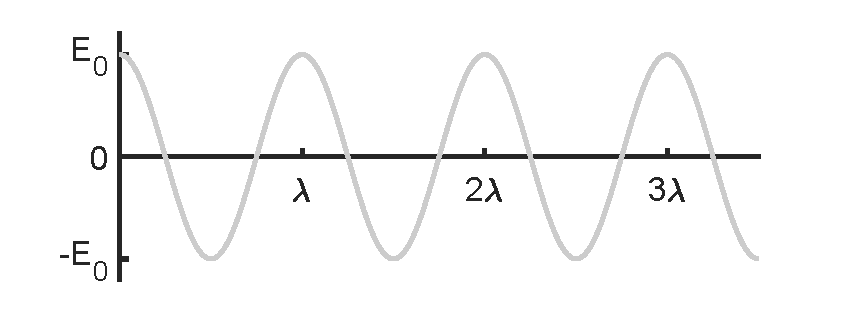
\includegraphics[width=0.6\textwidth]{\figpath/Model1_shiftedwave_blank.pdf}}
				}
				\centerline{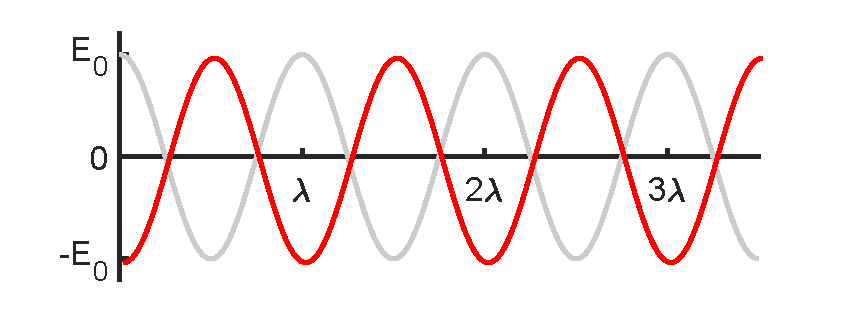
\includegraphics[width=0.6\textwidth]{\figpath/Model1_shiftedwave_solution.pdf}}
				\end{solution}
			
			\item Does shifting the wave change change either its amplitude or its wavelength?  Briefly explain how you know.
			
				\begin{solution}[1.5in]{}
					No, shifting the wave does not change either its amplitude or its wavelength.  The height of the peaks (the amplitude) remains unchanged, as does the distance between successive maxima of the wave.
				\end{solution}
				
		\end{enumerate}

	\question Mathematically, the electric field of an electromagnetic wave propagating along the $x$ axis can be expressed as
	\begin{equation*}
		E = E_0 \cos\left( \frac{2\pi x}{\lambda} + \delta \right)
	\end{equation*}
	In this expression, which variable ($E_0$, $\lambda$, or $\delta$) controls...
	
		\begin{enumerate}
		
			\item ... the amplitude of the wave?
			
				\begin{solution}[0.25in]{}
					$E_0$
				\end{solution}
			
			\item ... the wavelength of the wave?
			
				\begin{solution}[0.25in]{}
					$\lambda$
				\end{solution}
			
			\item ... the shift in the position of the wave?
			
				\begin{solution}[0.25in]{}
					$\delta$
				\end{solution}
		
		\end{enumerate}
		
\end{ctqs}

\begin{infobox}
	When the amplitudes of two electromagnetic waves measured at the same position have the \emph{same} sign, we refer to those waves as \emph{in phase} with each other.
	
	When the amplitudes of two electromagnetic waves measured at the same position have \emph{different} signs, we refer to those waves as \emph{out-of-phase} with each other.
\end{infobox}

\begin{ctqs}

	\question Two pairs of electromagnetic waves are shown below:
	
		\vspace{6pt}
		\begin{solution}[1.5in]{
			\centerline{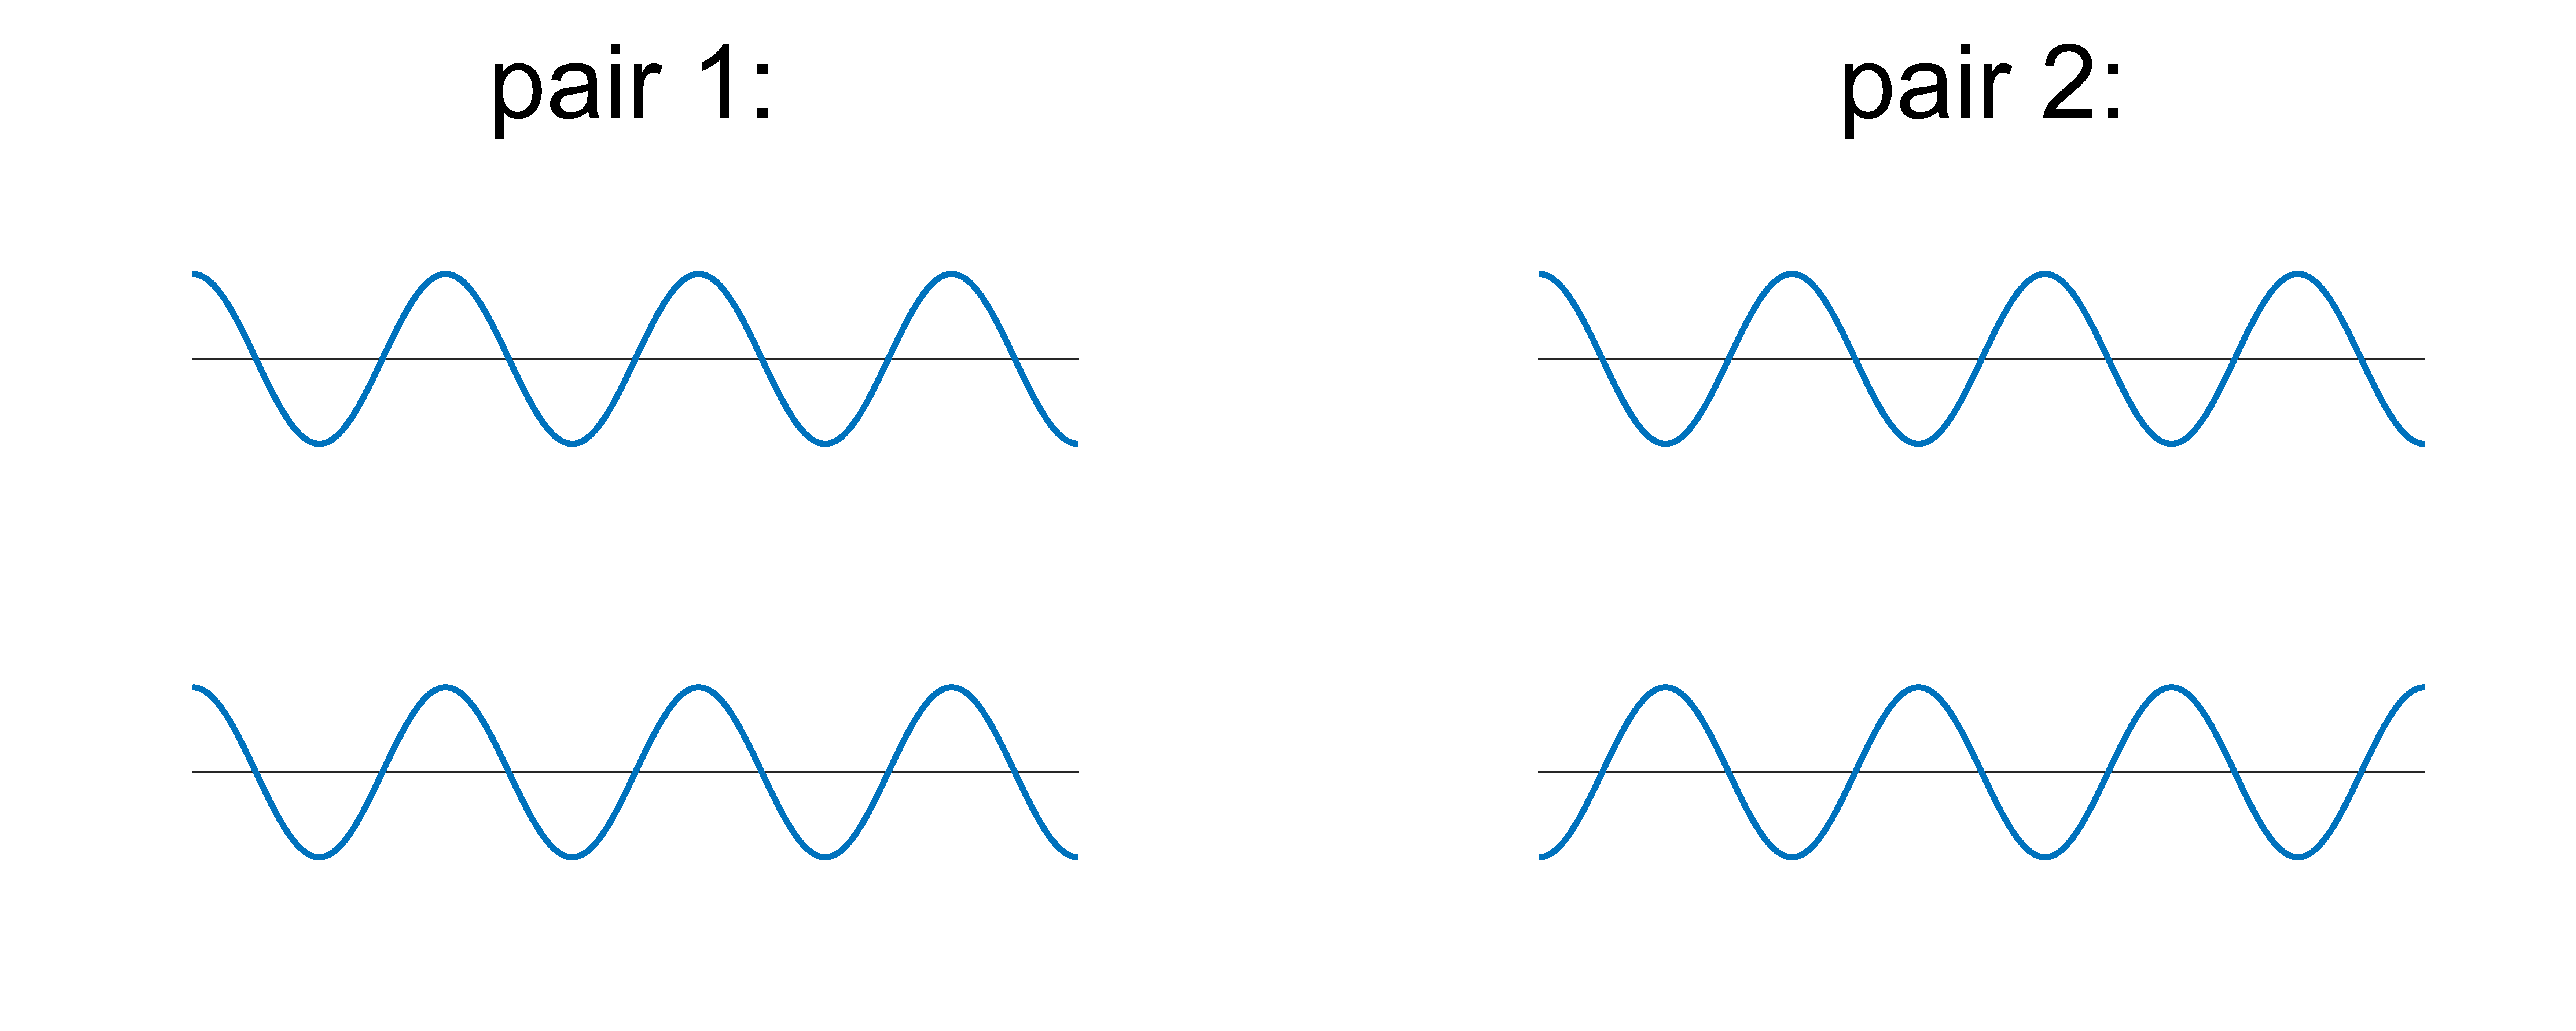
\includegraphics[width=0.7\textwidth]{\figpath/Model1_phasepairs}}
		}
			\centerline{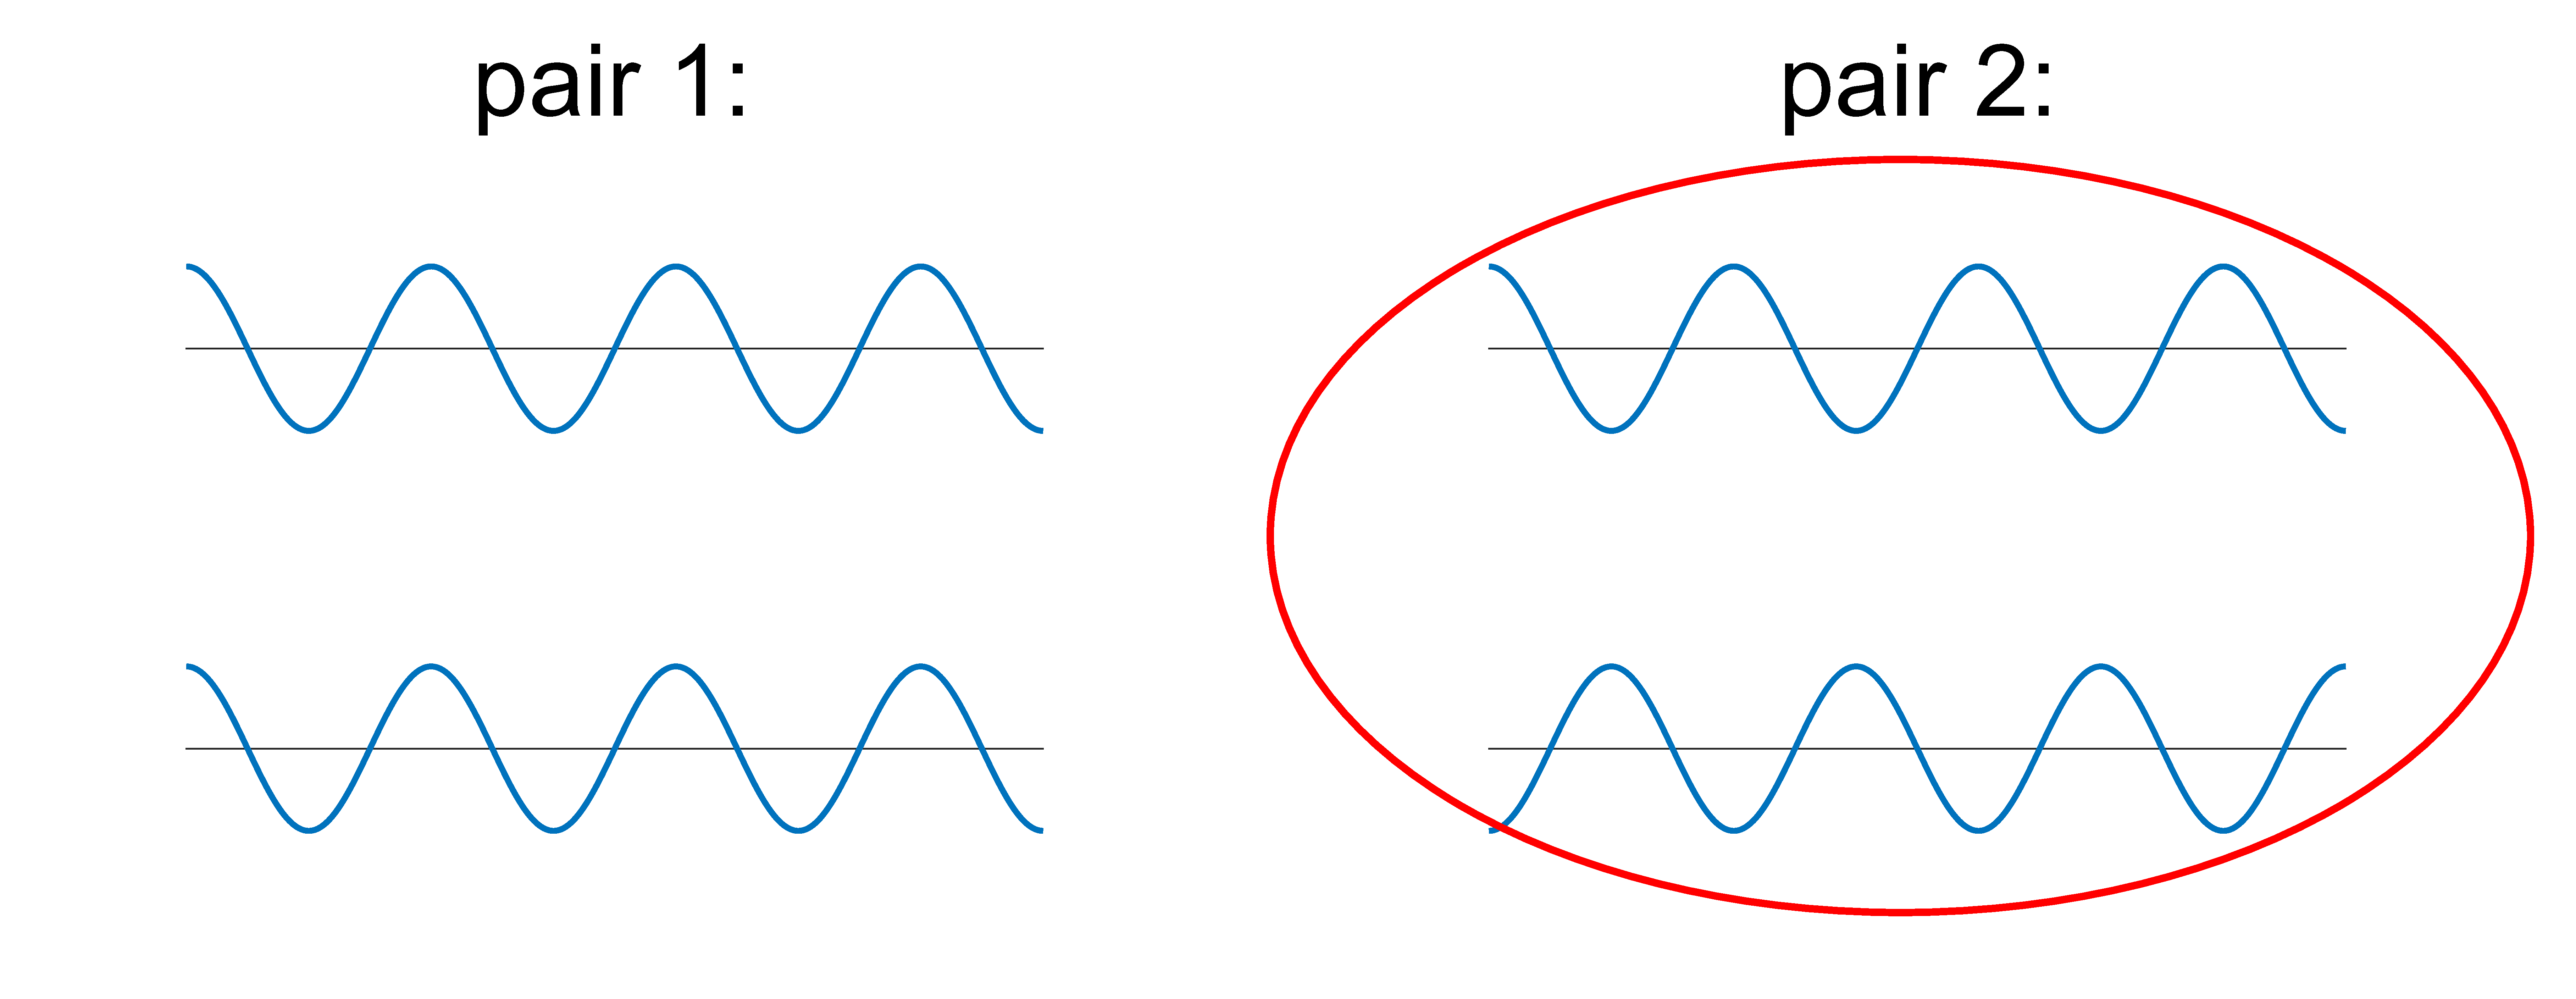
\includegraphics[width=0.7\textwidth]{\figpath/Model1_phasepairs_solution}}
		\end{solution}
		
		Circle the pair of waves that is \emph{out} of phase.
		
	\question When two waves are travelling together, their electric fields can be \emph{added} together to obtain the total electric field at each position.
	
		Predict the total electric field as a function of the spatial position $x$ for each of the pairs of waves shown in the previous question.
		
		\begin{solution}[1in]{
			\centerline{
\includegraphics[width=0.75\textwidth]{\figpath/Model1_wavesums_blank}}
		}
			\centerline{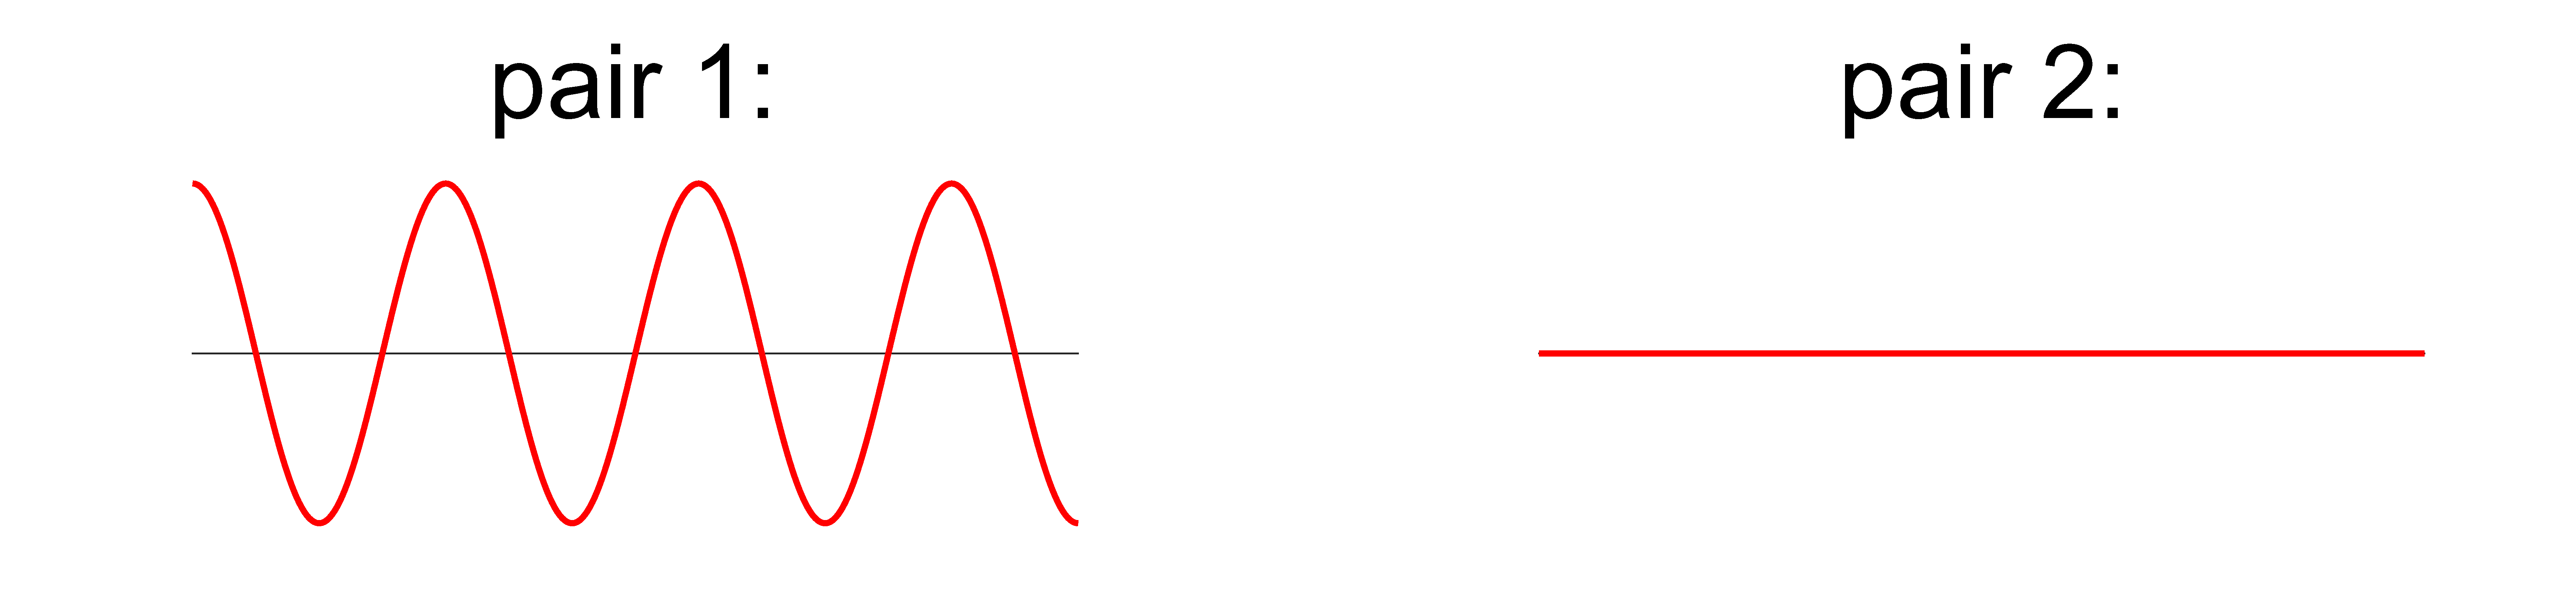
\includegraphics[width=0.7\textwidth]{\figpath/Model1_wavesums_solutions}}
		\end{solution}
		
	\question Most detectors, including cameras and human eyes, detect only the \emph{intensity} of an electromagetic wave.  The intensity of a wave is the square magnitude of the electric field, or
	\begin{equation*}
		I = |E|^2
	\end{equation*}
	
		Based on this information, and your answer to the previous question, would you expect to detect any signal from a pair of out-of-phase waves incident on a detector?  What about from a pair of in-phase waves?  Explain your group's reasoning in 1-2 complete sentences.
		
		\begin{solution}[2in]{}
			We should not detect any signal from a pair of out-of-phase waves incident on a detector.  As shown in the previous question, when two out-of-phase waves are summed together, the total electric field is zero.  Squaring zero still yields zero, so we will detect zero intensity.
			
			We \emph{should}, on the other hand, detect a signal from a pair of in-phase waves incident on a detector.  Summing two in-phase waves results in a wave with twice the amplitude of the original waves.  If we square this new wave, we will get a nonzero intensity.
			
			Note: while not addressed here, $E$ is typically complex, hence the need for the square magnitude when calculating intensity.
		\end{solution}

\end{ctqs}

\clearpage
\begin{model}[Scattering from Multiple Particles]
\label{\labelbase:mdl:twoparticlescattering}
	
	In scattering experiments, waves originating from the same source scatter off of different particles, and take different paths to the detector.  This process is shown for waves scattering off of two particles separated by distance $d$ at angle $\theta$, below:
	
	\vspace{6pt}
	\centerline{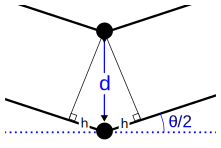
\includegraphics[width=0.8\textwidth]{\figpath/Model2_schematic}}
	
\end{model}

\begin{ctqs}

	\question As drawn, which wave travels the longer distance from the source to the detector?
	
		\begin{solution}[0.25in]{}
			wave 2
		\end{solution}
	
	\question As drawn, are the waves in-phase or out-of-phase when they exit the source?
	
		\begin{solution}[0.25in]{}
			in-phase
		\end{solution}
	
	\question As drawn, are the waves in-phase or out-of-phase when they reach the detector?
	
		\begin{solution}[0.25in]{}
			out-of-phase
		\end{solution}
	
	\question Explain, in 1-2 complete sentences, why the relative phase between the two waves at the detector depends on the difference in the lengths of the paths traveled by wave 1 and wave 2.
	
		\begin{solution}[2in]{}
			The phase of the waves oscillates as a function of $x$, or the distance traveled.  If two waves with the same wavelength start in-phase and travel exactly the same distance, then they will still be in phase by the time they reach the detector.  If one wave travels a slightly larger distance, however, its phase will continue to change over that extra distance, and it may no longer be in phase with the other wave by the time it reaches the detector.  The amount of ``extra'' phase change picked up by the second wave depends on how much extra distance it travels.
		\end{solution}
	
	\question For the geometry shown in Model \ref{\labelbase:mdl:twoparticlescattering}, it is possible to show %(see Exercise \ref{\labelbase:exc:deltax}) % SEE EXERCISE...
		that the difference in the path lengths of the two waves is \label{\labelbase:ctq:deltax}
		\begin{equation*}
			\Delta x = 2 d \sin\left(\frac{\theta}{2}\right)
		\end{equation*}
		
		Determine whether the waves will be in-phase or out-of-phase at the detector for each of the following values of $\Delta x$:
		
		\begin{enumerate}
			\item $\Delta x = 0$:
				\begin{solution}[0.25in]{}
					in phase
				\end{solution}
			\item $\Delta x = \lambda/2$:
				\begin{solution}[0.25in]{}
					out of phase
				\end{solution}
			\item $\Delta x = \lambda$:
				\begin{solution}[0.25in]{}
					in phase
				\end{solution}
			\item $\Delta x = 3\lambda/2$:
				\begin{solution}[0.25in]{}
					out of phase
				\end{solution}
		\end{enumerate}
		
	\question Generalizing your results above, explain why the signal measured on a detector will be largest when $\Delta x = \lambda n$, where $n$ is an integer.
	
		\begin{solution}[1.5in]{}
			Wave 2 repeats itself and returns to being in phase with wave 1 every time the path length increases by $\lambda$.  Thus, when the difference in path lengths is an integer multiple of lambda, the two waves will be in phase with each other at the detector, resulting in constructive interference and a large measured intensity.  When the difference in path lengths is \textit{not} an integer multiple of $\lambda$, some destructive interference occurs, decreasing the measured intensity. 
		\end{solution}
	
	\question In many scattering experiments, the wavelength $\lambda$ is fixed, and the scattered intensity is measured as a function of the scattering angle, $\theta$.  Setting the equations for $\Delta x$ from the previous two questions equal to each other and rearranging, we find that the maximum signal occurs at angles
		\begin{align*}
			\sin \frac{\theta}{2} = \frac{\lambda n}{2d} && \text{or} && \theta = 2\sin^{-1}\left(\frac{\lambda n}{2d}\right)
		\end{align*}
		Mark the angles at which the maximum intensity would be measured for particles separated by each of the following distances, assuming the scattering experiment is conducted using light with a wavelength of $\lambda=500\text{ nm}$: \label{\labelbase:ctq:scattangles}
		
		\begin{solution}[1.5in]{
			\centerline{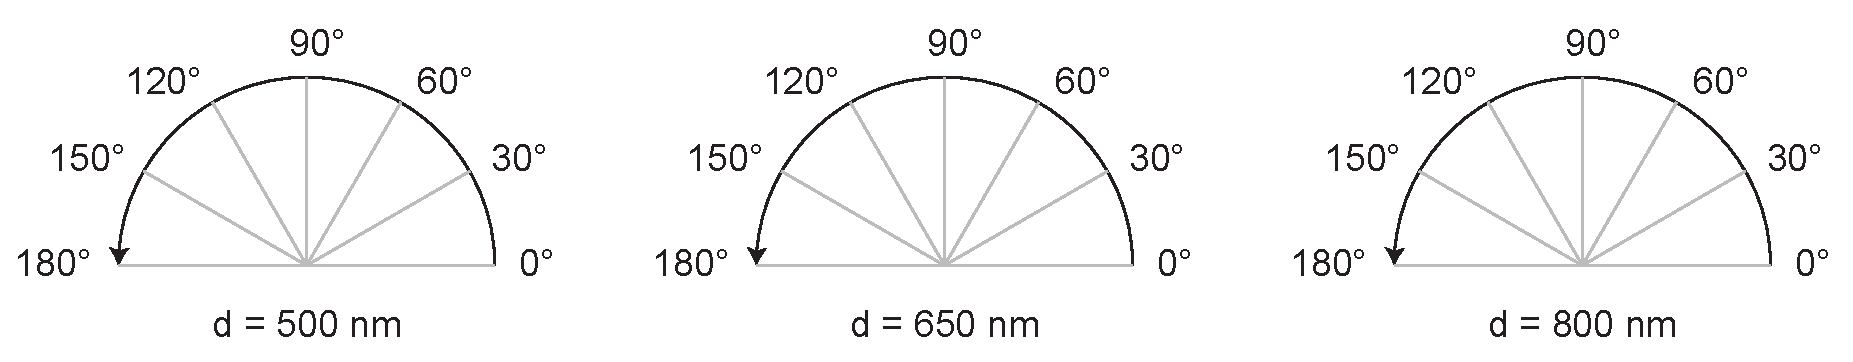
\includegraphics[width=\textwidth]{\figpath/Model2_theta_d_blank.pdf}}
		}
			\centerline{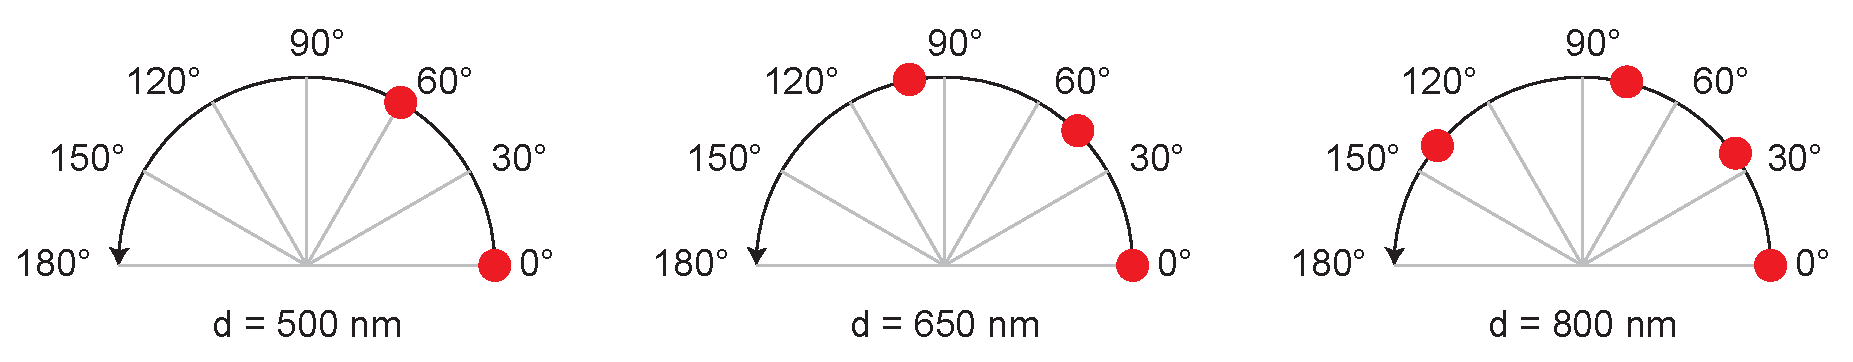
\includegraphics[width=\textwidth]{\figpath/Model2_theta_d_solutions.pdf}}
		\end{solution}
		
	\question Explain, in 2-3 complete sentences, how scattering experiments could be used to obtain information about the distances between different particles in a sample.
	
		\begin{solution}[2in]{}
			To obtain information about the distances between different particles in a sample, we could do the following:
			\begin{enumerate}
				\item Measure the intensity as a function of scattering angle
				\item Identify the angle(s) at which peaks (or maxima) in the scattered intensity are observed
				\item Calculate the particle spacing using $d = \frac{\lambda n}{2\sin(\theta/2)}$, where the peak observed at the smallest non-zero angle has $n=1$, the peak at the next angle has $n=2$, etc.
			\end{enumerate}
		\end{solution}
	
	\question Would a scattering experiment conducted using light with $\lambda=500\text{ nm}$ give useful information about the distance between the particles if $d$ were very small (say, $d=1\text{ nm}$) or very large (e.g. $d=100~\mu\text{m}$?  Explain your group's reasoning in 2-3 complete sentences.
	
		\begin{solution}[1.75in]{}
			No, a scattering experiment conducted using light with $\lambda=500\text{ nm}$ would probably not give useful information about the distance between the particles when $d=1\text{ nm}$ or $d=100~\mu\text{m}$.
			
			When $d$ is very small, $\frac{\lambda}{2d}$ is large.  Once $\frac{\lambda}{2d}>1$, we can no longer compute the inverse sine of this function, so there will be no solutions for $\theta$ in the equations given in CTQ \ref{\labelbase:ctq:scattangles}.  As a result, we will only see a peak at $\theta=0$ and nowhere else, so we will not obtain any information about the value of $d$ (except that it is small).
			
			When $d$ is very large, $\frac{\lambda n}{2d}$ will be small for many values of $n$.  As a result, the scattering peaks will be very close together, at small angles, and might not be possible to measure individually.
		\end{solution}
	
\end{ctqs}

\begin{model}[The Scattering Vector]
	\label{\labelbase:mdl:scatteringvector}
	
	A more general version of the scattering experiment shown in Model \ref{\labelbase:mdl:twoparticlescattering} is shown below:
	
	\centerline{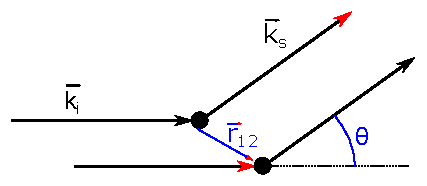
\includegraphics[width=0.4\textwidth]{\figpath/Model3_schematic.pdf}}
	
	Here, vectors $\vec k_i$ and $\vec k_s$ are the \emph{wavevectors} pointing in the directions of the incident and scattered waves, $\vec r_{12}$ is the vector between the two particles, and $\theta$ is the angle between the incident and scattered waves.
	
	In this geometry, it is possible to show (see Exercise \ref{\labelbase:exc:scatteringvector}) that the difference in the path lengths of the two waves is
	\begin{equation*}
		\Delta x = \vec r_{12}\cdot \frac{\vec k_i - \vec k_s}{|\vec k|}
	\end{equation*}
	
	
\end{model}

\begin{ctqs}
	
	\question The vector $\vec k_i - \vec k_s$ is referred to as the \emph{scattering vector}, $\vec q$.  Sketch the scattering vector for each of the following pairs of $\vec k_i$ and $\vec k_s$:
		
		\begin{solution}[1.5in]{\centerline{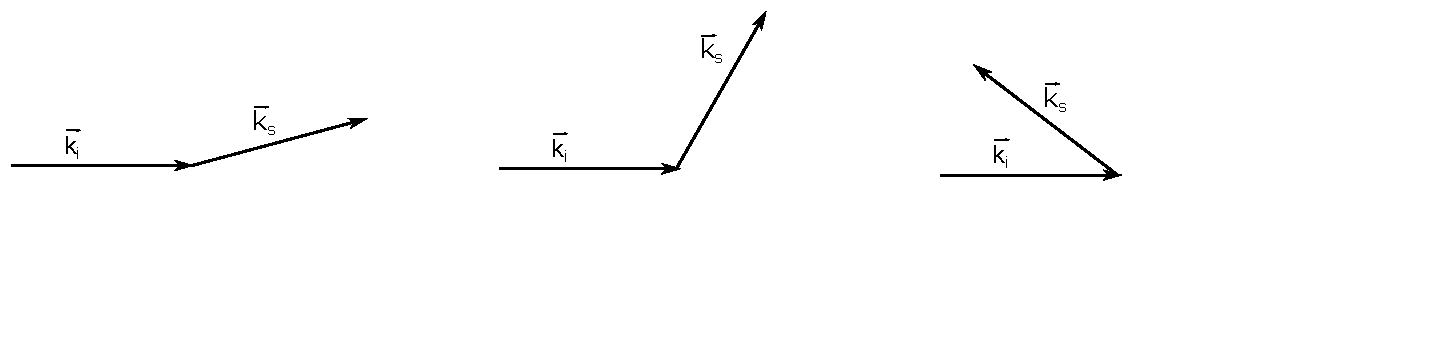
\includegraphics[width=\textwidth]{\figpath/Model3_qvecs_blank}}}
			\centerline{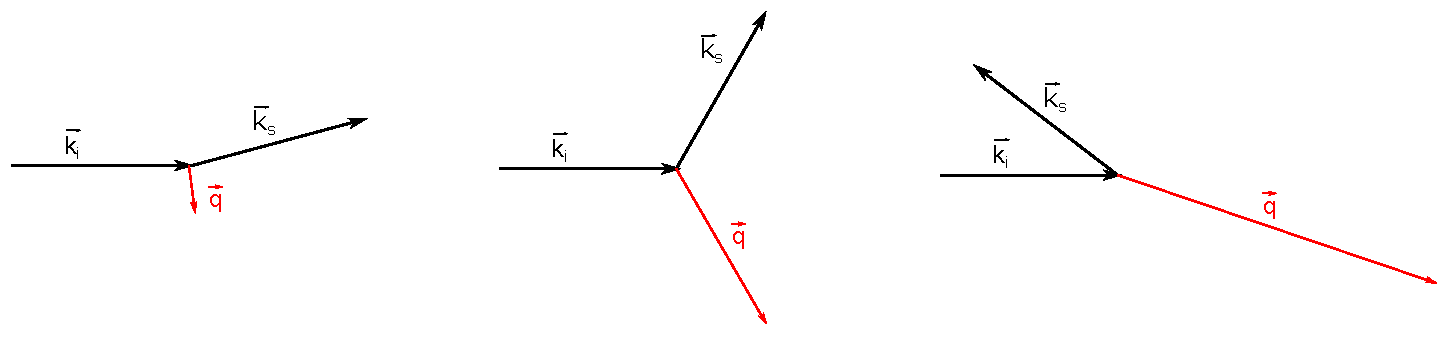
\includegraphics[width=\textwidth]{\figpath/Model3_qvecs_solutions}}
		\end{solution}
		
	\question How is the \emph{length} of the scattering vector related to the \emph{angle} between the incident and scattered waves?  Summarize your observations in 1-2 complete sentences.
		
		\begin{solution}[1.25in]{}
			The length of the scattering vector increases as the scattering angle $\theta$ increases.
		\end{solution}
		
	\question It is possible to show that the scattering vector has magnitude \label{\labelbase:ctq:magq}
	\begin{equation*}
		|\vec q| = 2\left(\frac{2\pi}{\lambda}\right)\sin\left(\frac{\theta}{2}\right)
	\end{equation*}
		Is this equation consistent with your answer to the previous question?  Explain your reasoning in 1-2 complete sentences.
		
		\begin{solution}[1in]{}
			Yes, this equation is consistent with the answers to the previous question.  As the scattering angle increases, $\sin\left(\frac{\theta}{2}\right)$ increases.  This in turn increases the value of $|\vec q|$, which corresponds to increasing the length of the scattering vector.
		\end{solution}

	\question Why might it be reasonable to plot data from a scattering experiment as a function of $|\vec q|$ rather than as a function of $\theta$?  Explain your reasoning in 1-2 complete sentences.
	
		\begin{solution}[1in]{}
			$|\vec q|$ increases monotonically as the scattering angle does.  Thus, it can just be used as a proxy for the scattering angle.  Either one is a reasonable variable to use.
		\end{solution}
		

\end{ctqs}

\begin{infobox}

%	The magnitude of the wavevector is related to the wavelength of the wave by $|\vec k| = \frac{2\pi}{\lambda}$.  Combining this expression with the equations in the previous question, it can be shown that a peak at scattering vector $|\vec q|$ corresponds to a particle spacing of
	It is possible to show (see Exercise \ref{\labelbase:exc:rq}) that a peak in the scattering intensity at scattering vector $|\vec q|$ corresponds to a particle spacing of \label{\labelbase:eqn:rq}
		\begin{align*}
			|\vec r| = \frac{2\pi}{|\vec q|}
		\end{align*}
		
\end{infobox}

\begin{ctqs}

	\question Typical wavelengths and scattering angles for common scattering experiments are given below.  Using the equation given above (along with the equation for $|\vec q|$ on the previous page), calculate the range of particle spacings that should be measurable in each experiment. \label{\labelbase:ctq:calcrranges}

%	\begin{center}
%	\renewcommand{\arraystretch}{1.3}
%	\begin{tabular}{ccc}
%		\hline
%		\textbf{Experiment} & \textbf{Wavelength ($\lambda$)} & \textbf{Angles ($\theta$)}\\\hline
%		Light Scattering & 400-700~nm & 20-160${}^\circ$ \\
%		Small-Angle X-ray Scattering (SAXS) & 0.05-0.2~nm & 0.1-5${}^\circ$\\ 
%		Wide-Angle X-ray Scattering (WAXS) & 0.5-1.8~\AA & 5-60${}^\circ$\\
%		Small-Angle Neutron Scattering (SANS) & 4-20~\AA & 0.1-3${}^\circ$\\\hline
%	\end{tabular}
%	\end{center}

	\begin{enumerate}
		\item \textbf{Light scattering:} $\lambda = 633$~nm and $\theta = 30-150^\circ$
		
			\begin{solution}[2.75in]{}
				To make this problem easier, note that
				\begin{align*}
					|\vec r| &= \frac{2\pi}{|\vec q|} = \frac{2\pi}{2\left(\frac{2\pi}{\lambda}\right)\sin\left(\frac{\theta}{2}\right)} 
				= \frac{\lambda}{2\sin\left(\frac{\theta}{2}\right)}
				\end{align*}
				Substituting in $\lambda = 633$~nm and $\theta=30^\circ$:
				\begin{equation*}
					|\vec r| = \frac{633\text{ nm}}{2\sin(15^\circ)} = 1200\text{ nm} = 1.2~\mu\text{m}
				\end{equation*}
				Substituting in $\lambda = 633$~nm and $\theta=150^\circ$:
				\begin{equation*}
					|\vec r| = \frac{633\text{ nm}}{2\sin(75^\circ)} = 330\text{ nm}
				\end{equation*}
				Thus light scattering should be sensitive to spacings/displacements of approximately 300-1200~nm.
			\end{solution}
		
		\item \textbf{Small-angle X-ray scattering (SAXS):} $\lambda = 0.15$~nm and $\theta = 0.1-5^\circ$
		
			\begin{solution}[2.75in]{}
				Substituting in $\lambda = 0.15$~nm and $\theta=0.1^\circ$:
				\begin{equation*}
					|\vec r| = \frac{0.15\text{ nm}}{2\sin(0.05^\circ)} = 85~\text{nm}
				\end{equation*}
				Substituting in $\lambda = 0.15$~nm and $\theta=5^\circ$:
				\begin{equation*}
					|\vec r| = \frac{0.15\text{ nm}}{2\sin(2.5^\circ)} = 1.7~\text{nm}
				\end{equation*}
				Thus SAXS should be sensitive to spacings/displacements of approximately 2-80~nm.
			\end{solution}
		
		\item \textbf{Wide-angle X-ray scattering (WAXS):} $\lambda = 0.15$~nm and $\theta = 5-60^\circ$
		
			\begin{solution}[2.5in]{}
				Substituting in $\lambda = 0.15$~nm and $\theta=5^\circ$:
				\begin{equation*}
					|\vec r| = \frac{0.15\text{ nm}}{2\sin(2.5^\circ)} = 1.7~\text{nm}
				\end{equation*}
				Substituting in $\lambda = 0.15$~nm and $\theta=60^\circ$:
				\begin{equation*}
					|\vec r| = \frac{0.15\text{ nm}}{2\sin(30^\circ)} = 0.15~\text{nm}
				\end{equation*}
				Thus WAXS should be sensitive to spacings/displacements of approximately 0.1-2~nm.
			\end{solution}
		
		\item \textbf{Small-angle neutron scattering (SANS):} $\lambda = 1$~nm and $\theta = 0.1-3^\circ$
		
			\begin{solution}[2.5in]{}
				Substituting in $\lambda = 1$~nm and $\theta=0.1^\circ$:
				\begin{equation*}
					|\vec r| = \frac{1\text{ nm}}{2\sin(0.05^\circ)} = 530~\text{nm}
				\end{equation*}
				Substituting in $\lambda = 1$~nm and $\theta=3^\circ$:
				\begin{equation*}
					|\vec r| = \frac{1\text{ nm}}{2\sin(1.5^\circ)} = 20~\text{nm}
				\end{equation*}
				Thus WAXS should be sensitive to spacings/displacements of approximately 20-500~nm.
			\end{solution}
		
	\end{enumerate}

	\question Based on your calculations, which type(s) of experiment(s) would be most suitable for measuring each of the following features or processes in polymer systems?  Briefly indicate your reasoning for each item. \label{\labelbase:ctq:exptchoices}
	
		\begin{enumerate}
		
			\item The radius of gyration of a polymer chain
			
				\begin{solution}[0.75in]{}
					Radii of gyration of polymer chains are typically on the order of 10s of nm.  SAXS and SANS are well-suited to measuring these values.  (Note: light scattering can also be used to determine $R_g$, but students do not have enough information to figure this out yet - see the next activity.)
				\end{solution}
			
			\item The characteristic domain spacing of a block copolymer
			
				\begin{solution}[0.75in]{}
					Block copolymers typically have domain spacings on the order of 10s of nm.  SAXS and SANS are, again, both able to measure these values (though SAXS is typically used because it is higher resolution and does not require expensive deuteration of the polymer).
				\end{solution}
				
			\item The arrangement of atoms in a polyethylene crystal
			
				\begin{solution}[0.5in]{}
					Atoms in polymer crystals are typically separated by distances of a few angstroms.  WAXS is the best technique for measuring features on this length scale.
				\end{solution}
			
			\item The diffusion of a polymer micelle over a distance of $\sim 1~\mu$m
			
				\begin{solution}[0.5in]{}
					Light scattering is best suited to measuring processes that happen on length scales of $\sim 1~\mu$m.
				\end{solution}
			
		\end{enumerate}
	
\end{ctqs}


\begin{exercises}

	\exercise The scattering geometry shown in Model \ref{\labelbase:mdl:twoparticlescattering} can be re-drawn as follows: \label{\labelbase:exc:deltax}
		
		\vspace{6pt}
	\centerline{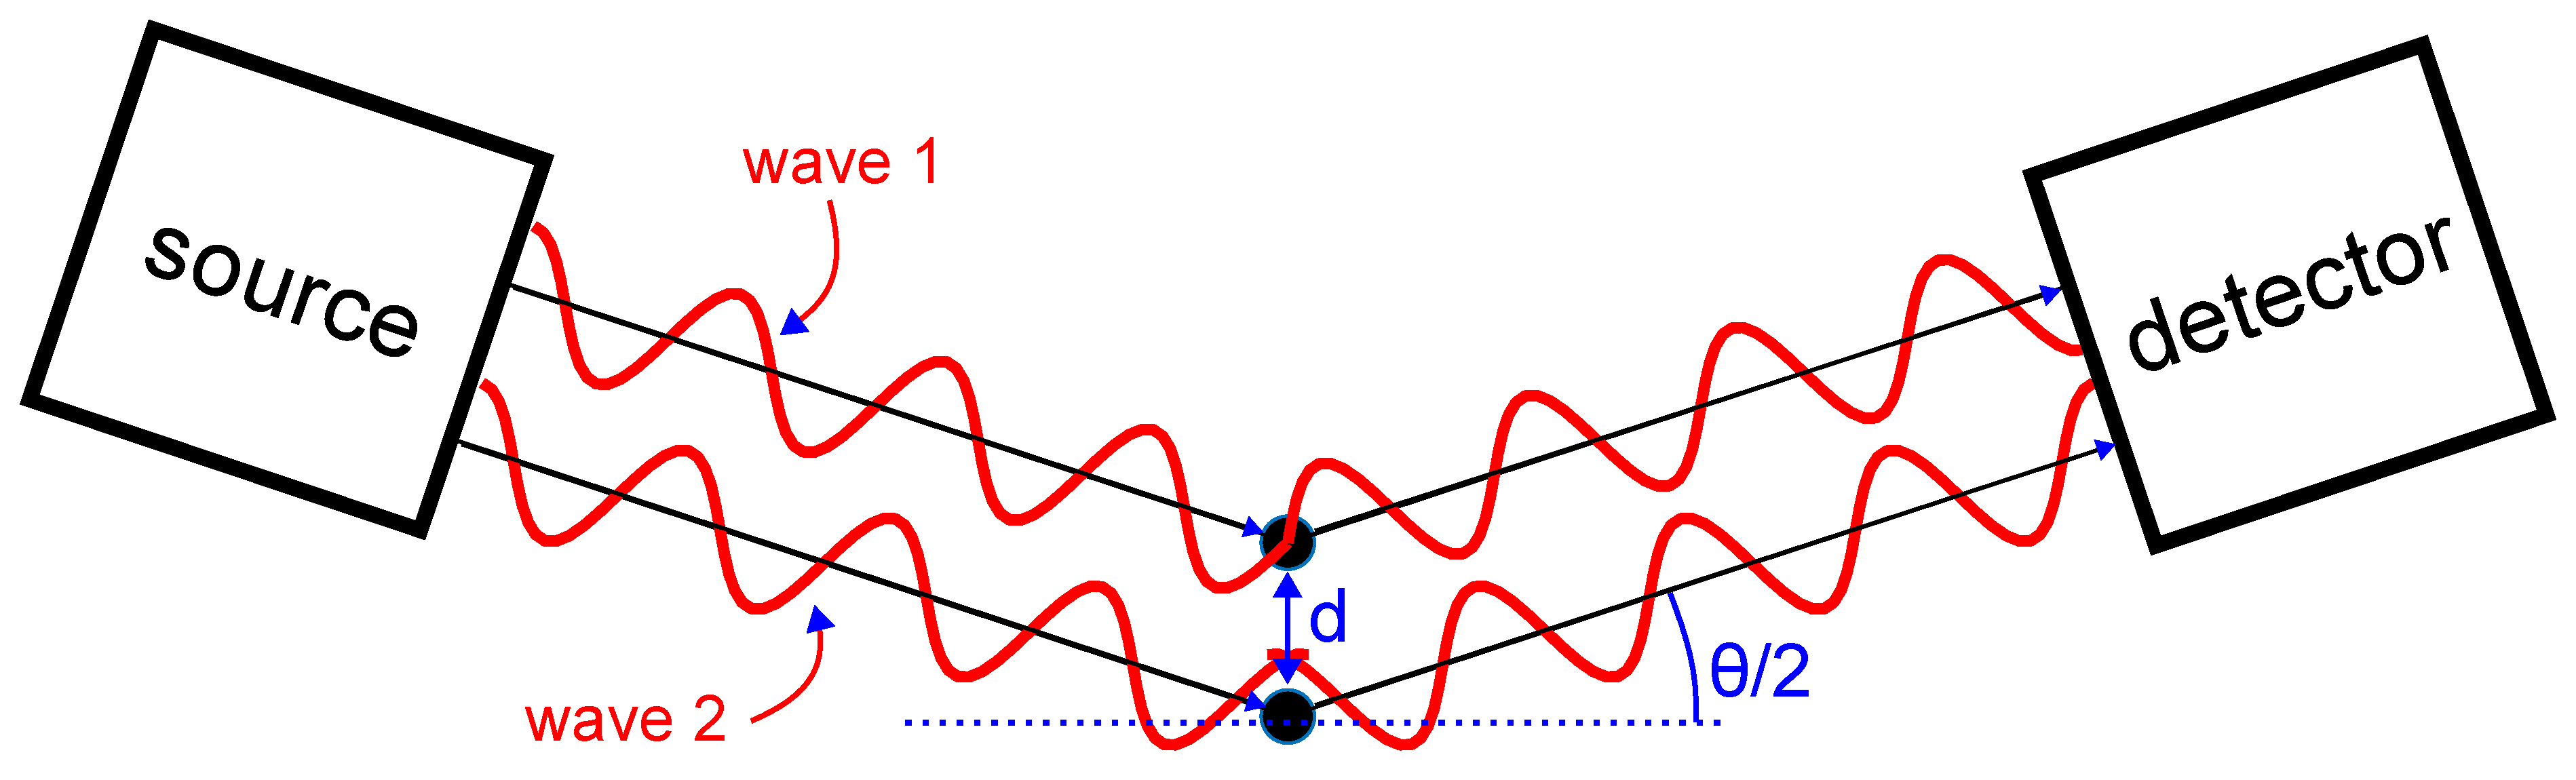
\includegraphics[width=0.6\textwidth]{\figpath/Model2_schematic_theta2}}
	
	``Zooming in'' on the two scattering centers, this scattering geometry is
		
		\vspace{6pt}	
	\centerline{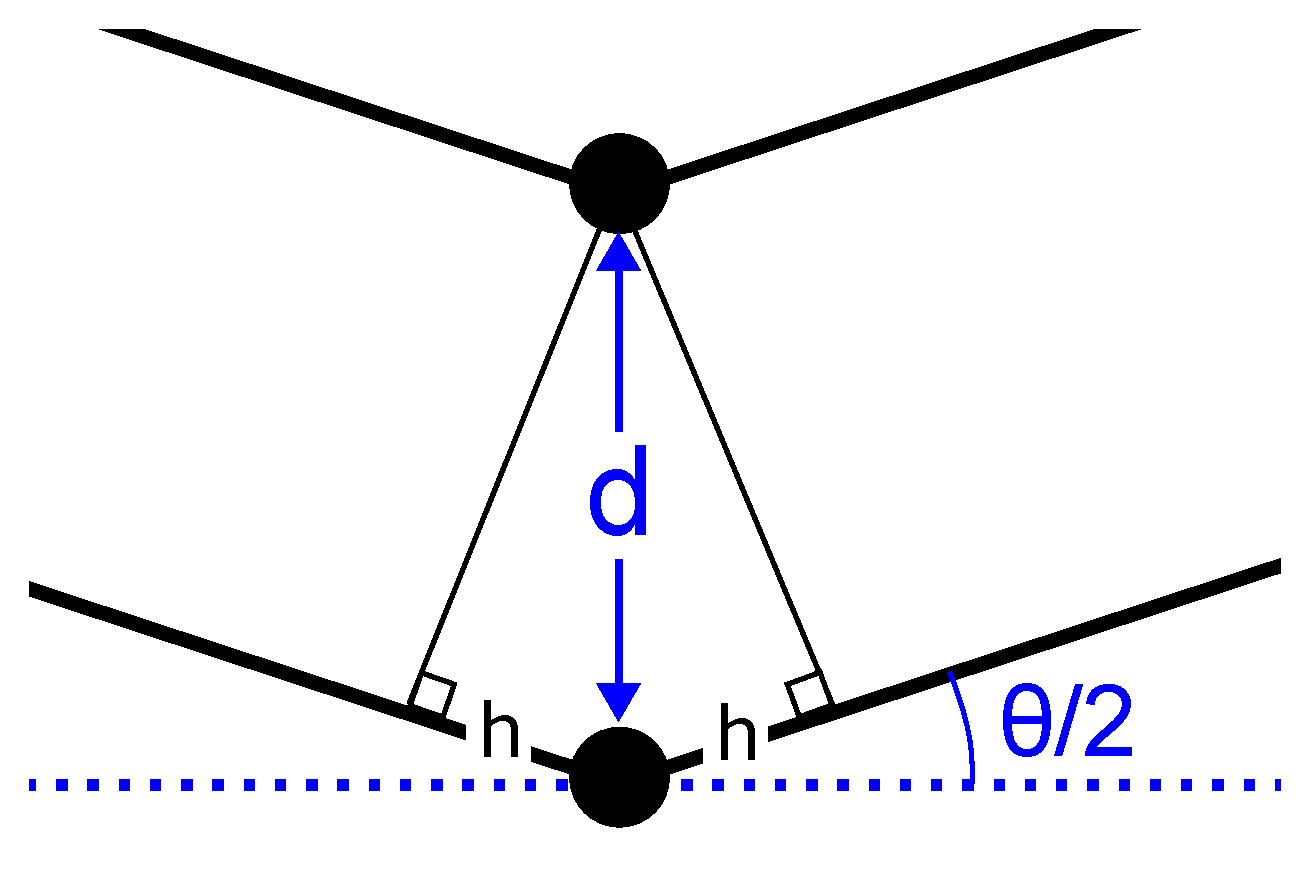
\includegraphics[width=0.3\textwidth]{\figpath/Model2_schematic_theta2_zoom}}
	
	\begin{enumerate}
		\item Explain, in 2-3 complete sentences, why the difference in the path lengths traveled by wave 1 and wave 2 is $2h$.
		
			\begin{solution}{}
				The relative phase of the waves is the same as long as they are traveling on perfectly parallel paths.  On the left-hand side, the waves are in phase until wave 1 hits the top particle.  At this point, however, wave 2 still needs to travel distance $h$ to hit the bottom particle.  On the right-hand side, wave 2 then needs to travel another distance $h$ before it ``catches up'' with the path of wave 1 and returns to traveling parallel to wave 1.  Wave 2 thus travels an extra distance of $2h$ compared to wave 1.
			\end{solution}
		
		\item Find an expression for $h$ in terms of $d$ and $\theta/2$, and verify that it yields the same value of $\Delta x$ given in CTQ \ref{\labelbase:ctq:deltax}.
		
			\begin{solution}{}
				In the geometry shown, the angle between vector $d$ and the outgoing wave is $90^\circ-\theta/2$.  The angle between vector $d$ and the line drawn perpendicular to the wave paths is then $90^\circ - (90^\circ-\theta/2) = \theta/2$.  The sine of this angle is $h/d$, so
				\begin{equation*}
					\frac{h}{d} = \sin\left(\frac{\theta}{2}\right)
				\end{equation*}
				The extra distance traveled by wave 2 is thus
				\begin{equation*}
					\Delta x = 2h = 2 d\sin\left(\frac{\theta}{2}\right)
				\end{equation*}
				exactly as given in CTQ \ref{\labelbase:ctq:deltax}.
			\end{solution}
	\end{enumerate}

	\exercise Justify the expression for $\Delta x$ given in Model \ref{\labelbase:mdl:scatteringvector} by doing the following: \label{\labelbase:exc:scatteringvector}
	
		\begin{enumerate}
			\item Write an expression for the projection of $\vec r_{12}$ onto $\vec k_i$.
			
				\begin{solution}{}
					The projection of vector $\vec a$ onto $\vec b$ is
					\begin{equation*}
						proj_b a = \frac{\vec a \cdot \vec b}{|\vec b|^2} \vec b
					\end{equation*}
					The projection of $\vec r_{12}$ onto $\vec k_i$ is thus
					\begin{equation*}
						\frac{\vec r \cdot \vec k_i}{|\vec k_i|^2} \vec k_i
					\end{equation*}
				\end{solution}
				
			\item Write an expression for the projection of $\vec r_{12}$ onto $\vec k_s$.
			
				\begin{solution}{}
					As above, the projection of $\vec r_{12}$ onto $\vec k_s$ is
					\begin{equation*}
						\frac{\vec r \cdot \vec k_s}{|\vec k_s|^2} \vec k_s
					\end{equation*}
				\end{solution}
			
			\item Re-draw the figure from Model \ref{\labelbase:mdl:scatteringvector}, and add both of the vectors calculated in parts (a) and (b).  Explain, in 2-3 complete sentences, why the the difference in the path lengths of the two waves is given by the difference of these lengths of these vectors.
			
				\begin{solution}{}
					The relevant figure is
					
					\centerline{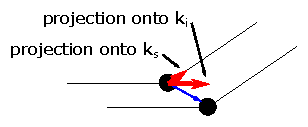
\includegraphics[width=0.5\textwidth]{\figpath/Model3_projections}}
					
					Moving these vectors around a little bit, we see that the length of the projection of $\vec r$ onto $\vec k_i$ is the amount of extra distance traveled by the bottom wave to reach the the particle before it scatters, while the length of the projection of $\vec r$ onto $\vec k_s$ is the amount of extra distance traveled by the top wave to reach the detector after it scatters
					
					\centerline{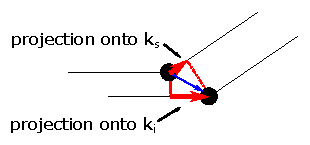
\includegraphics[width=0.5\textwidth]{\figpath/Model3_projections2}}
					
					The difference between these values gives the \emph{net} extra distance traveled by wave 2 to reach the detector.
					
				\end{solution}
			
			
			\item Verify that taking this difference yields the expression given in Model \ref{\labelbase:mdl:scatteringvector}.
			
				\begin{solution}{}
				
					We want to subtract the lengths of the vectors, not the vectors themselves.  It turns out that since $\frac{\vec b}{|\vec b|}$ is a unit vector, the (signed) length of $proj_b a$ is just $\frac{\vec a \cdot \vec b}{|\vec b|}$.
					
					Thus, the difference in the path lengths is just the difference in the (signed) lengths of the vectors found in parts (a) and (b), or
					\begin{equation*}
						\Delta x = \frac{\vec r \cdot \vec k_i}{|\vec k_i|} - \frac{\vec r \cdot \vec k_s}{|\vec k_s|}
					\end{equation*}
					Because $\vec k_i$ and $\vec k_s$ have the same wavelength, $|\vec k_i| = |\vec k_s| \equiv |\vec k|$, so
					\begin{align*}
						\Delta x &= \frac{\vec r \cdot \vec k_i}{|\vec k|} - \frac{\vec r \cdot \vec k_s}{|\vec k|}\\
							&= \vec r_{12} \cdot \frac{\vec k_i - \vec k_s}{|\vec k|}
					\end{align*}
					as given in the model.
					
				\end{solution}
			
			
		\end{enumerate}
	
	\exercise Show that if $|\vec k_i| = |\vec k_s| = \frac{2\pi}{\lambda}$, then $|\vec q| = 2\left(\frac{2\pi}{\lambda}\right)\sin\left(\frac{\theta}{2}\right)$ as given on page \pageref{\labelbase:ctq:magq}. \label{\labelbase:ctq:magq}
	
		\begin{solution}{}
			Without loss of generality, we can define the wavevectors as follows:
			\begin{align*}
				\vec k_i &= \frac{2\pi}{\lambda}(\cos\frac{\theta}{2},-\sin\frac{\theta}{2})\\
				\vec k_s &= \frac{2\pi}{\lambda}(\cos\frac{\theta}{2},\sin\frac{\theta}{2})
			\end{align*}
			The scattering vector is then
			\begin{align*}
				\vec q = \vec k_i - \vec k_s = \frac{2\pi}{\lambda}(0,2\sin\frac{\theta}{2})
			\end{align*}
			and its magnitude is
			\begin{align*}
				|\vec q| &= \frac{2\pi}{\lambda}\sqrt{ 0^2 + \left(2\sin\frac{\theta}{2}\right)^2}\\
				&= \frac{2\pi}{\lambda}\left(2\sin\frac{\theta}{2}\right)\\
				&= 2\left(\frac{2\pi}{\lambda}\right)\sin\left(\frac{\theta}{2}\right)
			\end{align*}
			as desired.
			
			Note: this problem is can also be done by defining the vectors as 
			\begin{align*}
				\vec k_i &= \frac{2\pi}{\lambda}(1,0)\\
				\vec k_s &= \frac{2\pi}{\lambda}(\cos\theta,\sin\theta)
			\end{align*}
			However, the math then requires use of a half-angle formula to obtain the final expression in terms of $\sin\frac{\theta}{2}$, so it is easier to set the calculation up as above.
		\end{solution}
	
	\exercise Justify the expression for $|\vec r|$ given on page \pageref{\labelbase:eqn:rq} by doing the following: \label{\labelbase:exc:rq}
	
		\begin{enumerate}
			\item Rewrite the expression for $\Delta x$ given in Model \ref{\labelbase:mdl:scatteringvector} in terms of $\vec q$.
			
				\begin{solution}{}
					\begin{equation*}
						\Delta x = \frac{\vec r_{12} \cdot \vec q}{|\vec k|}
					\end{equation*}
				\end{solution}
			
			\item When two vectors are parallel, their dot product is just the product of their magnitudes.  Using this information, rewrite your expression for $\Delta x$ in terms of the magnitudes of $\vec r$, $\vec q$, and $\vec k$ for the case in which $\vec r$ and $\vec q$ point in the same direction.
			
				\begin{solution}{}
					\begin{equation*}
						\Delta x = \frac{|\vec r_{12}| |\vec q|}{|\vec k|}
					\end{equation*}
				\end{solution}
			
			\item What is the smallest nonzero value of $\Delta x$ that will ensure the scattered waves are in phase when they reach the detector (hint: look back at CTQ \ref{\labelbase:ctq:deltax})?  Set your expression for $\Delta x$ equal to this value and solve for $|\vec r|$.
			
				\begin{solution}{}
					The smallest nonzero value of $\Delta x$ that will ensure the scattered waves are in phase when they reach the detector is $\Delta x=\lambda$.  Substituting this in and rearranging, we have
					\begin{align*}
						\lambda &= \frac{|\vec r_{12}| |\vec q|}{|\vec k|}\\
						|\vec r| &= \frac{\lambda |\vec k|}{|\vec q|}
					\end{align*}
				\end{solution}
			
			\item Finally, the magnitude of the wavevector is $\frac{2\pi}{\lambda}$.  Substitute this value into your expression from the previous part and verify that you obtain the equation given on page \pageref{\labelbase:eqn:rq}.
			
				\begin{solution}{}
					\begin{equation*}
						|\vec r| = \frac{\lambda \frac{2\pi}{\lambda}}{|\vec q|} = \frac{2\pi}{|\vec q|}
					\end{equation*}
					(which does indeed match the equation given in the activity)
				\end{solution}
			
			\item This derivation made the assumption that $\vec r$ and $\vec q$ point in the same direction.  Will this always be true?  If not, why might it still be reasonable to use this expression to determine the particle spacing from the value of $|\vec q|$ at which the maximum intensity is observed? Explain your reasoning in 2-3 complete sentences.
			
			\begin{solution}{}
		
				No, this will not always be true.  The direction of $\vec q$ is set by the measurement geometry (i.e. the angle at which we have placed our detector relative to the incident beam).  Thus, it may not always be the same as the direction of $\vec r$, which depends only on the arrangement of particles in the sample, not the detection angle.
				
				%The reason that this calculation still generally works is that the distribution of inter-particle vectors is usually \textit{isotropic} (i.e. it is, on average, random and uniform).  When we take the average over all of these vectors, the part of the signal that ``survives'' and is detected is the part satisfying $|\vec r| = \frac{\lambda \frac{2\pi}{\lambda}}{|\vec q|} = \frac{2\pi}{|\vec q|}$.
			\end{solution}
		
		\end{enumerate}
	
\end{exercises}


%\begin{problems}
%
%	\problem Derive the expression for $\Delta x$ in Model 2
%	
%\end{problems}


	
\end{activity}


\end{document}
